% Guia de início rápido do IPTV, edição em português. Compilar nesta pasta com:
%   pdflatex IPTV-Quick-Start-pt.tex   (duas vezes, para o índice)
\newcommand{\GuideLang}{portuguese}
\newcommand{\GuideTitle}{Guia de início rápido}
\newcommand{\TipLabel}{Dica.}
% Shared layout of the IPTV quick start guides (one file per language:
% IPTV-Quick-Start.tex, IPTV-Quick-Start-it.tex, ...). Each sets, before
% % Shared layout of the IPTV quick start guides (one file per language:
% IPTV-Quick-Start.tex, IPTV-Quick-Start-it.tex, ...). Each sets, before
% % Shared layout of the IPTV quick start guides (one file per language:
% IPTV-Quick-Start.tex, IPTV-Quick-Start-it.tex, ...). Each sets, before
% \input{preamble}:
%   \GuideLang   babel language (english, italian, spanish, french, ngerman, portuguese)
%   \GuideTitle  the guide's title, used on the cover, in headers and the PDF
%   \TipLabel    the word that starts a tip box ("Tip.")
% Build any of them with pdflatex, twice (for the table of contents).
\documentclass[11pt,a4paper]{article}

\usepackage[T1]{fontenc}
\usepackage[utf8]{inputenc}
% shorthands=off: no language-specific active characters (they would clash
% with tables and addresses); only hyphenation and "Contents" etc. change.
\usepackage[shorthands=off,\GuideLang]{babel}
\usepackage{lmodern}
\usepackage[scaled=0.92]{helvet}
\renewcommand{\familydefault}{\sfdefault}
\usepackage[margin=2.2cm,headheight=14pt]{geometry}
\usepackage{graphicx}
\usepackage[table]{xcolor}
\usepackage{booktabs}
\usepackage{tabularx}
\usepackage{xltabular}
\usepackage{enumitem}
\usepackage{titlesec}
\usepackage{fancyhdr}
\usepackage{pifont}
\usepackage{amssymb}
\usepackage[hidelinks]{hyperref}

\newcommand{\version}{0.12}
\definecolor{accent}{HTML}{1E6FD9}
\definecolor{dim}{HTML}{5F6673}
\definecolor{notebg}{HTML}{EEF4FC}
\definecolor{warnbg}{HTML}{FFF6E0}
\definecolor{tvred}{HTML}{D32F2F}
\definecolor{tvgreen}{HTML}{2E7D32}
\definecolor{tvyellow}{HTML}{C9A400}
\definecolor{tvblue}{HTML}{1565C0}

\hypersetup{pdftitle={IPTV -- \GuideTitle}, pdfauthor={IPTV project}}
\setlist{itemsep=2pt, topsep=4pt}
\setlength{\parindent}{0pt}
\setlength{\parskip}{6pt}
\renewcommand{\arraystretch}{1.25}

\titleformat{\section}{\Large\bfseries\color{accent}}{\thesection}{0.6em}{}
\titleformat{\subsection}{\large\bfseries}{\thesubsection}{0.6em}{}
\titlespacing*{\section}{0pt}{14pt}{6pt}
\titlespacing*{\subsection}{0pt}{10pt}{4pt}

\pagestyle{fancy}
\fancyhf{}
\fancyhead[L]{\small\color{dim}IPTV -- \GuideTitle}
\fancyhead[R]{\small\color{dim}github.com/vickdini/iptv}
\fancyfoot[C]{\small\color{dim}\thepage}
\renewcommand{\headrulewidth}{0.4pt}
\renewcommand{\sectionmark}[1]{\markboth{#1}{}}

% A key or button on a keyboard / remote.
\newcommand{\key}[1]{{\setlength{\fboxsep}{1.5pt}\fbox{\footnotesize\vphantom{Ay}#1}}}
% A coloured remote button.
\newcommand{\colorkey}[2]{\textcolor{#1}{\ding{108}}\,\textbf{#2}}
% Shaded boxes for tips and notes.
\newcommand{\tip}[1]{\par\noindent\colorbox{notebg}{\parbox{\dimexpr\linewidth-2\fboxsep}{\small\textbf{\TipLabel} #1}}\par}
\newcommand{\note}[1]{\par\noindent\colorbox{warnbg}{\parbox{\dimexpr\linewidth-2\fboxsep}{\small #1}}\par}
\newcommand{\menu}[1]{\textit{#1}}
\newcommand{\download}{\url{https://github.com/vickdini/iptv/releases/latest}}
% Key tables: \rowcolors{2}{gray!8}{white} then
% \begin{xltabular}{\linewidth}{@{}KX@{}} \keyshead{Key}{What it does} ... \bottomrule
\newcolumntype{K}{>{\raggedright\arraybackslash}p{5.4cm}}
\newcommand{\keyshead}[2]{\toprule \textbf{#1} & \textbf{#2} \\ \midrule}

% The cover: #1 subtitle, #2 "Version".
\newcommand{\cover}[2]{%
\begin{titlepage}
  \centering
  \vspace*{0.5cm}
  {\fontsize{40}{48}\selectfont\bfseries\color{accent} IPTV\par}
  \vspace{0.3cm}
  {\LARGE \GuideTitle\par}
  \vspace{0.3cm}
  {\large\color{dim} #1\par}
  \vspace{1cm}
  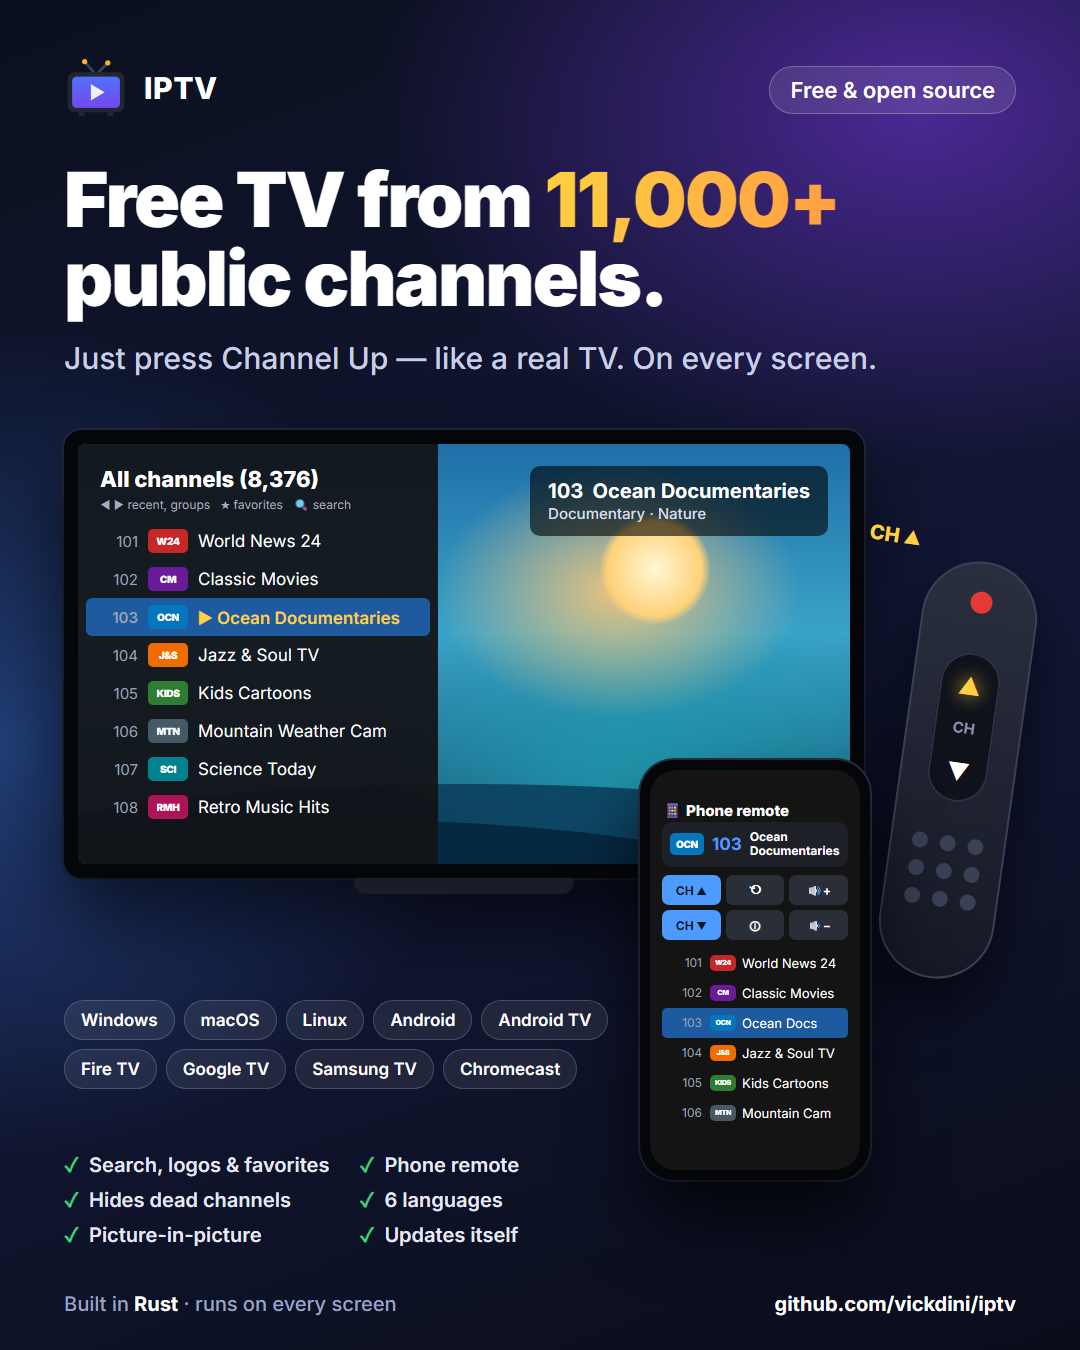
\includegraphics[width=0.52\textwidth]{../images/iptv-overview.png}\par
  \vfill
  {\large Windows \textbullet{} macOS \textbullet{} Linux \textbullet{} Android
   \textbullet{} Android TV \& Fire TV \textbullet{} Chromecast \textbullet{} Samsung TV\par}
  \vspace{0.5cm}
  {\color{dim} #2 \version{} \textbullet{} \url{https://github.com/vickdini/iptv}\par}
\end{titlepage}
\tableofcontents
\thispagestyle{fancy}}
:
%   \GuideLang   babel language (english, italian, spanish, french, ngerman, portuguese)
%   \GuideTitle  the guide's title, used on the cover, in headers and the PDF
%   \TipLabel    the word that starts a tip box ("Tip.")
% Build any of them with pdflatex, twice (for the table of contents).
\documentclass[11pt,a4paper]{article}

\usepackage[T1]{fontenc}
\usepackage[utf8]{inputenc}
% shorthands=off: no language-specific active characters (they would clash
% with tables and addresses); only hyphenation and "Contents" etc. change.
\usepackage[shorthands=off,\GuideLang]{babel}
\usepackage{lmodern}
\usepackage[scaled=0.92]{helvet}
\renewcommand{\familydefault}{\sfdefault}
\usepackage[margin=2.2cm,headheight=14pt]{geometry}
\usepackage{graphicx}
\usepackage[table]{xcolor}
\usepackage{booktabs}
\usepackage{tabularx}
\usepackage{xltabular}
\usepackage{enumitem}
\usepackage{titlesec}
\usepackage{fancyhdr}
\usepackage{pifont}
\usepackage{amssymb}
\usepackage[hidelinks]{hyperref}

\newcommand{\version}{0.12}
\definecolor{accent}{HTML}{1E6FD9}
\definecolor{dim}{HTML}{5F6673}
\definecolor{notebg}{HTML}{EEF4FC}
\definecolor{warnbg}{HTML}{FFF6E0}
\definecolor{tvred}{HTML}{D32F2F}
\definecolor{tvgreen}{HTML}{2E7D32}
\definecolor{tvyellow}{HTML}{C9A400}
\definecolor{tvblue}{HTML}{1565C0}

\hypersetup{pdftitle={IPTV -- \GuideTitle}, pdfauthor={IPTV project}}
\setlist{itemsep=2pt, topsep=4pt}
\setlength{\parindent}{0pt}
\setlength{\parskip}{6pt}
\renewcommand{\arraystretch}{1.25}

\titleformat{\section}{\Large\bfseries\color{accent}}{\thesection}{0.6em}{}
\titleformat{\subsection}{\large\bfseries}{\thesubsection}{0.6em}{}
\titlespacing*{\section}{0pt}{14pt}{6pt}
\titlespacing*{\subsection}{0pt}{10pt}{4pt}

\pagestyle{fancy}
\fancyhf{}
\fancyhead[L]{\small\color{dim}IPTV -- \GuideTitle}
\fancyhead[R]{\small\color{dim}github.com/vickdini/iptv}
\fancyfoot[C]{\small\color{dim}\thepage}
\renewcommand{\headrulewidth}{0.4pt}
\renewcommand{\sectionmark}[1]{\markboth{#1}{}}

% A key or button on a keyboard / remote.
\newcommand{\key}[1]{{\setlength{\fboxsep}{1.5pt}\fbox{\footnotesize\vphantom{Ay}#1}}}
% A coloured remote button.
\newcommand{\colorkey}[2]{\textcolor{#1}{\ding{108}}\,\textbf{#2}}
% Shaded boxes for tips and notes.
\newcommand{\tip}[1]{\par\noindent\colorbox{notebg}{\parbox{\dimexpr\linewidth-2\fboxsep}{\small\textbf{\TipLabel} #1}}\par}
\newcommand{\note}[1]{\par\noindent\colorbox{warnbg}{\parbox{\dimexpr\linewidth-2\fboxsep}{\small #1}}\par}
\newcommand{\menu}[1]{\textit{#1}}
\newcommand{\download}{\url{https://github.com/vickdini/iptv/releases/latest}}
% Key tables: \rowcolors{2}{gray!8}{white} then
% \begin{xltabular}{\linewidth}{@{}KX@{}} \keyshead{Key}{What it does} ... \bottomrule
\newcolumntype{K}{>{\raggedright\arraybackslash}p{5.4cm}}
\newcommand{\keyshead}[2]{\toprule \textbf{#1} & \textbf{#2} \\ \midrule}

% The cover: #1 subtitle, #2 "Version".
\newcommand{\cover}[2]{%
\begin{titlepage}
  \centering
  \vspace*{0.5cm}
  {\fontsize{40}{48}\selectfont\bfseries\color{accent} IPTV\par}
  \vspace{0.3cm}
  {\LARGE \GuideTitle\par}
  \vspace{0.3cm}
  {\large\color{dim} #1\par}
  \vspace{1cm}
  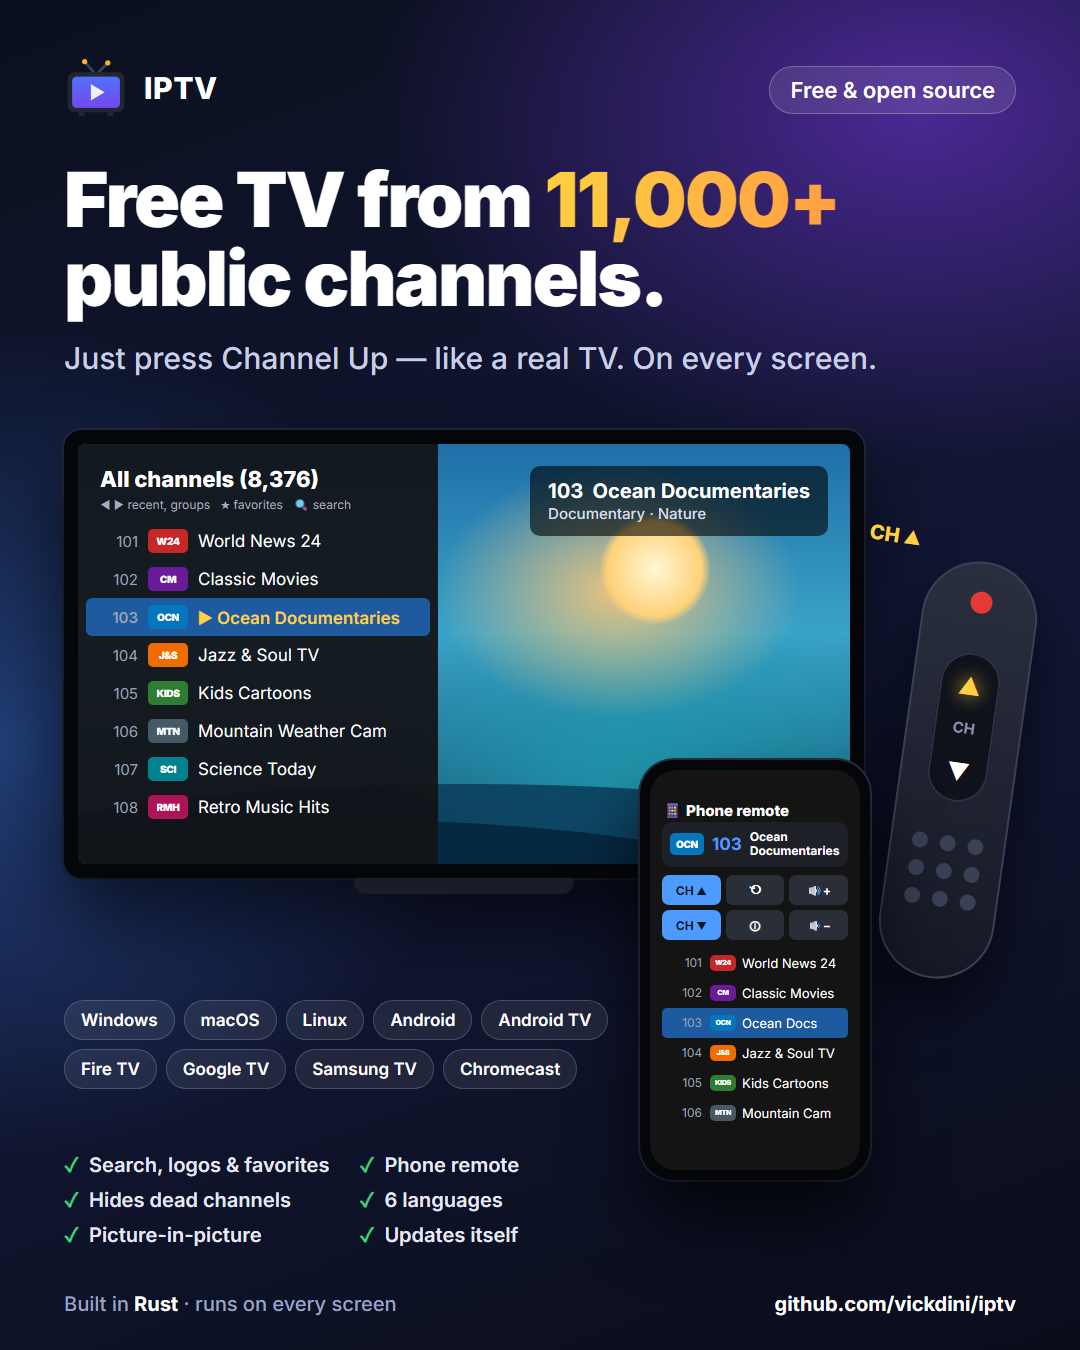
\includegraphics[width=0.52\textwidth]{../images/iptv-overview.png}\par
  \vfill
  {\large Windows \textbullet{} macOS \textbullet{} Linux \textbullet{} Android
   \textbullet{} Android TV \& Fire TV \textbullet{} Chromecast \textbullet{} Samsung TV\par}
  \vspace{0.5cm}
  {\color{dim} #2 \version{} \textbullet{} \url{https://github.com/vickdini/iptv}\par}
\end{titlepage}
\tableofcontents
\thispagestyle{fancy}}
:
%   \GuideLang   babel language (english, italian, spanish, french, ngerman, portuguese)
%   \GuideTitle  the guide's title, used on the cover, in headers and the PDF
%   \TipLabel    the word that starts a tip box ("Tip.")
% Build any of them with pdflatex, twice (for the table of contents).
\documentclass[11pt,a4paper]{article}

\usepackage[T1]{fontenc}
\usepackage[utf8]{inputenc}
% shorthands=off: no language-specific active characters (they would clash
% with tables and addresses); only hyphenation and "Contents" etc. change.
\usepackage[shorthands=off,\GuideLang]{babel}
\usepackage{lmodern}
\usepackage[scaled=0.92]{helvet}
\renewcommand{\familydefault}{\sfdefault}
\usepackage[margin=2.2cm,headheight=14pt]{geometry}
\usepackage{graphicx}
\usepackage[table]{xcolor}
\usepackage{booktabs}
\usepackage{tabularx}
\usepackage{xltabular}
\usepackage{enumitem}
\usepackage{titlesec}
\usepackage{fancyhdr}
\usepackage{pifont}
\usepackage{amssymb}
\usepackage[hidelinks]{hyperref}

\newcommand{\version}{0.12}
\definecolor{accent}{HTML}{1E6FD9}
\definecolor{dim}{HTML}{5F6673}
\definecolor{notebg}{HTML}{EEF4FC}
\definecolor{warnbg}{HTML}{FFF6E0}
\definecolor{tvred}{HTML}{D32F2F}
\definecolor{tvgreen}{HTML}{2E7D32}
\definecolor{tvyellow}{HTML}{C9A400}
\definecolor{tvblue}{HTML}{1565C0}

\hypersetup{pdftitle={IPTV -- \GuideTitle}, pdfauthor={IPTV project}}
\setlist{itemsep=2pt, topsep=4pt}
\setlength{\parindent}{0pt}
\setlength{\parskip}{6pt}
\renewcommand{\arraystretch}{1.25}

\titleformat{\section}{\Large\bfseries\color{accent}}{\thesection}{0.6em}{}
\titleformat{\subsection}{\large\bfseries}{\thesubsection}{0.6em}{}
\titlespacing*{\section}{0pt}{14pt}{6pt}
\titlespacing*{\subsection}{0pt}{10pt}{4pt}

\pagestyle{fancy}
\fancyhf{}
\fancyhead[L]{\small\color{dim}IPTV -- \GuideTitle}
\fancyhead[R]{\small\color{dim}github.com/vickdini/iptv}
\fancyfoot[C]{\small\color{dim}\thepage}
\renewcommand{\headrulewidth}{0.4pt}
\renewcommand{\sectionmark}[1]{\markboth{#1}{}}

% A key or button on a keyboard / remote.
\newcommand{\key}[1]{{\setlength{\fboxsep}{1.5pt}\fbox{\footnotesize\vphantom{Ay}#1}}}
% A coloured remote button.
\newcommand{\colorkey}[2]{\textcolor{#1}{\ding{108}}\,\textbf{#2}}
% Shaded boxes for tips and notes.
\newcommand{\tip}[1]{\par\noindent\colorbox{notebg}{\parbox{\dimexpr\linewidth-2\fboxsep}{\small\textbf{\TipLabel} #1}}\par}
\newcommand{\note}[1]{\par\noindent\colorbox{warnbg}{\parbox{\dimexpr\linewidth-2\fboxsep}{\small #1}}\par}
\newcommand{\menu}[1]{\textit{#1}}
\newcommand{\download}{\url{https://github.com/vickdini/iptv/releases/latest}}
% Key tables: \rowcolors{2}{gray!8}{white} then
% \begin{xltabular}{\linewidth}{@{}KX@{}} \keyshead{Key}{What it does} ... \bottomrule
\newcolumntype{K}{>{\raggedright\arraybackslash}p{5.4cm}}
\newcommand{\keyshead}[2]{\toprule \textbf{#1} & \textbf{#2} \\ \midrule}

% The cover: #1 subtitle, #2 "Version".
\newcommand{\cover}[2]{%
\begin{titlepage}
  \centering
  \vspace*{0.5cm}
  {\fontsize{40}{48}\selectfont\bfseries\color{accent} IPTV\par}
  \vspace{0.3cm}
  {\LARGE \GuideTitle\par}
  \vspace{0.3cm}
  {\large\color{dim} #1\par}
  \vspace{1cm}
  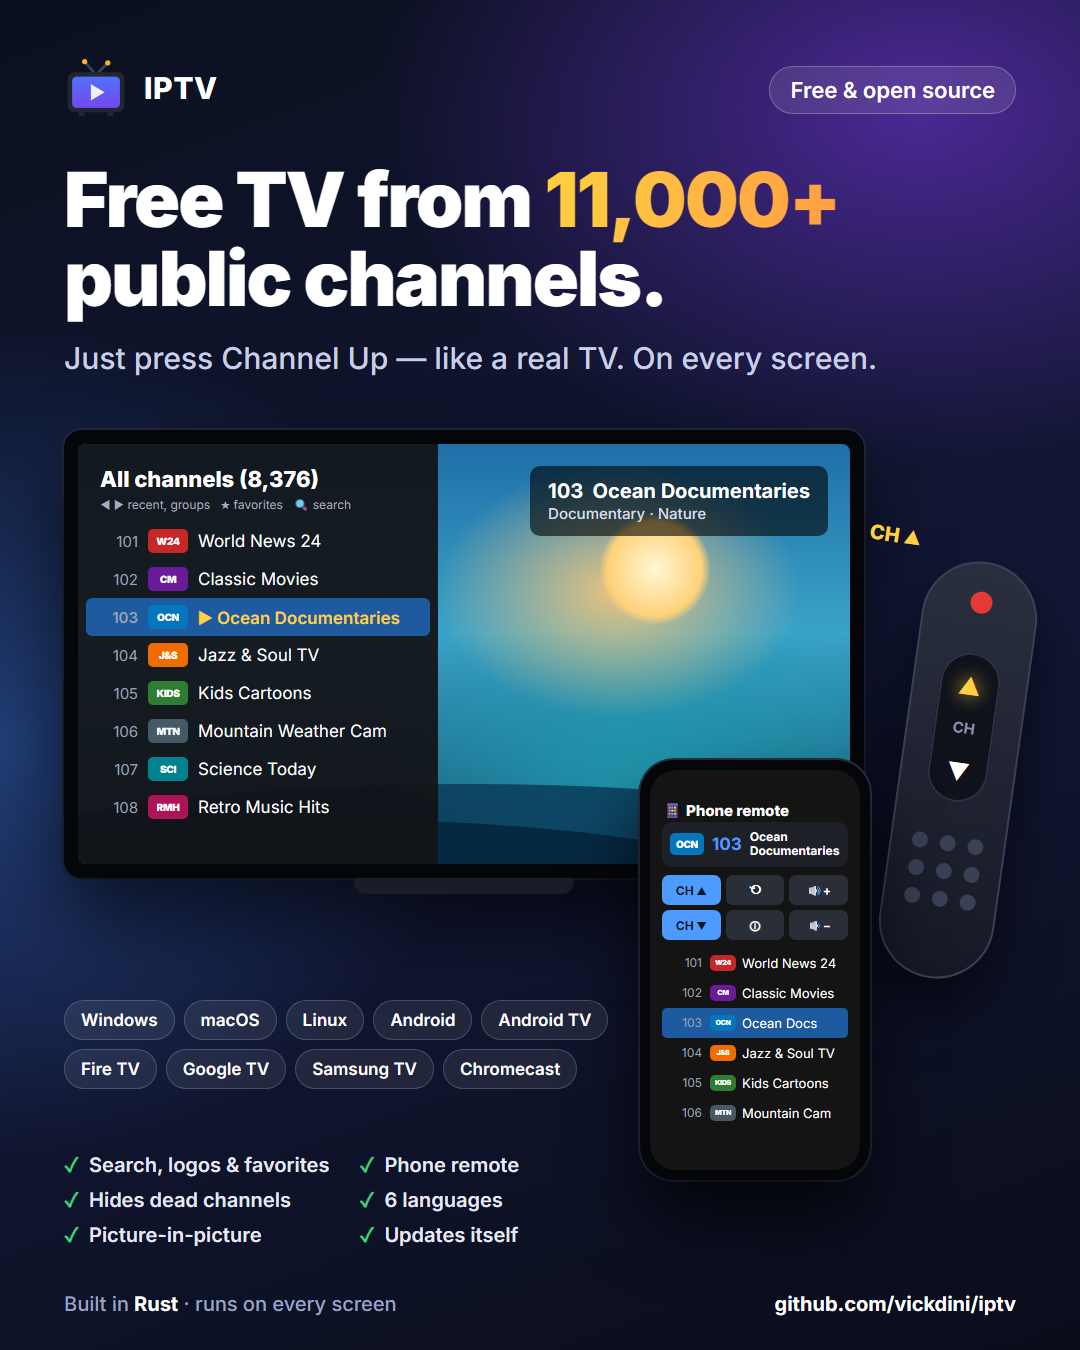
\includegraphics[width=0.52\textwidth]{../images/iptv-overview.png}\par
  \vfill
  {\large Windows \textbullet{} macOS \textbullet{} Linux \textbullet{} Android
   \textbullet{} Android TV \& Fire TV \textbullet{} Chromecast \textbullet{} Samsung TV\par}
  \vspace{0.5cm}
  {\color{dim} #2 \version{} \textbullet{} \url{https://github.com/vickdini/iptv}\par}
\end{titlepage}
\tableofcontents
\thispagestyle{fancy}}


\begin{document}
\cover{Veja canais de TV gratuitos e faça zapping como num televisor}{Versão}

% ------------------------------------------------------------------ intro
\section{O que é o IPTV}

O IPTV reproduz os canais de TV gratuitos e públicos reunidos pelo projeto
\emph{iptv-org} (mais de 10\,000) e permite-lhe mudar de um para outro como
num televisor: canal seguinte e anterior, números de canal, favoritos e
grupos como Notícias, Filmes ou Desporto.

\begin{itemize}
  \item \textbf{Sempre atualizado.} A lista de canais é atualizada sempre que
        o IPTV abre, e a aplicação atualiza-se sozinha quando sai uma versão
        nova.
  \item \textbf{Só canais que funcionam.} Os canais em baixo são escondidos
        automaticamente, por isso o zapping nunca para num ecrã preto.
  \item \textbf{Encontre canais depressa.} Pesquise pelo nome, reconheça cada
        canal pelo logótipo, volte aos canais vistos recentemente ou mostre
        só os países e idiomas que lhe interessam.
  \item \textbf{O seu idioma.} O IPTV fala português, inglês, italiano,
        espanhol, francês e alemão, e segue o idioma do seu dispositivo. Nos
        canais que os transmitem, escolha o idioma do áudio e ligue as
        legendas.
  \item \textbf{Comando no telemóvel.} Controle a TV ou o computador a partir
        do navegador do telemóvel (secção~\ref{sec:remote}).
\end{itemize}

Cada transferência inclui tudo o que é preciso: não há mais nada para
instalar. Todas as transferências estão na página de versões:

\begin{center}
  \download
\end{center}

\note{\textbf{Aviso.} O IPTV não aloja nem fornece nenhum vídeo: apenas
carrega uma lista pública publicada pelo projeto iptv-org. Veja apenas o que
a lei do seu país lhe permite ver.}

% ------------------------------------------------------------------ Windows
\section{Windows}
\label{sec:windows}

\subsection{Instalação}
\begin{enumerate}
  \item Transfira \texttt{IPTV-Setup-\textless versão\textgreater.exe} da
        página de versões e abra-o.
  \item Se o Windows mostrar \menu{O Windows protegeu o computador}, clique
        em \menu{Mais informações} e depois em \menu{Executar mesmo assim}.
  \item Siga o instalador. Não precisa de direitos de administrador e
        adiciona um atalho no menu Iniciar (e um ícone no ambiente de
        trabalho, se quiser).
\end{enumerate}
O IPTV abre maximizado e começa logo a reproduzir. Para o remover, use
\menu{Definições \textrightarrow{} Aplicações}.

\subsection{Teclas}
\label{sec:keys}
Estas teclas funcionam em todos os computadores: Windows, macOS e Linux.

\rowcolors{2}{gray!8}{white}
\begin{xltabular}{\linewidth}{@{}KX@{}}
\keyshead{Tecla}{O que faz}
\key{$\uparrow$} \key{$\downarrow$}, \key{PgUp} \key{PgDn}, roda do rato & canal seguinte / anterior \\
\key{0}--\key{9}, depois esperar ou \key{Enter} & ir para um número de canal \\
\key{Backspace} & voltar ao canal anterior \\
\key{$\leftarrow$} \key{$\rightarrow$}, \key{m} & baixar / subir o volume, sem som \\
\key{l}, \key{Tab} ou clique direito & abrir / fechar a lista de canais \\
\key{/} ou \key{Ctrl}+\key{F} & pesquisar canais pelo nome \\
\key{c} & escolher países e idiomas \\
\key{g} / \key{G} & vistos recentemente e depois os grupos (Notícias, Filmes\ldots) \\
\key{s} / \key{S} & marcar ou desmarcar um favorito / zapping só entre favoritos \\
\key{a} / \key{t} & idioma do áudio seguinte / legendas seguintes (e desligadas) \\
\key{r} & comando no telemóvel: mostrar o código QR \\
\key{E} / \key{I} & exportar / importar favoritos (pasta Transferências) \\
\key{i} & informações do canal \\
\key{f}, duplo clique & ecrã inteiro (\key{Esc} para sair) \\
\key{p} & imagem pequena: um segundo canal, pequeno, no canto inferior direito \\
\key{[} / \key{]} & canal anterior / seguinte da imagem pequena \\
\key{x}, clique na imagem pequena & trocar os dois canais \\
\key{Espaço} & pausa \\
\key{h}, \key{?} ou \key{F1} & ajuda no ecrã \\
\key{q} & sair \\
\bottomrule
\end{xltabular}

\subsection{A lista de canais}
Prima \key{l} para abrir à esquerda uma lista de canais com os seus
logótipos; o vídeo continua ao lado. Desloque-se com a roda do rato e clique
num canal para o ver. Comece a escrever (ou prima \key{/}) para pesquisar:
acentos e maiúsculas não importam. \key{Esc} fecha a lista. Prima \key{g}
para os canais vistos recentemente, do mais recente para o mais antigo.

\subsection{Países e idiomas}
Prima \key{c}, escreva para encontrar um país ou idioma e prima \key{Enter}
para o marcar; \key{Tab} muda entre as duas listas. A partir daí o IPTV só
mostra os canais dos países marcados ou nos idiomas marcados, até limpar a
escolha (\key{Del}, ou a linha \emph{Limpar todos os filtros}).

\subsection{Idioma do áudio e legendas}
Quando um canal oferece mais de um idioma de áudio ou legendas, uma nota no
fundo do ecrã indica-o. Prima \key{a} para o idioma do áudio seguinte e
\key{t} para as legendas seguintes (e por fim \emph{desligadas}). O IPTV
lembra-se do idioma e usa-o em todos os outros canais que o oferecem.

\subsection{Idioma e atualizações}
O IPTV usa o idioma do sistema. Sempre que abre, verifica se há uma versão
nova; se houver, instala-a sem perguntar e reinicia sozinho passados alguns
segundos.

% ------------------------------------------------------------------ macOS
\section{macOS}

\subsection{Instalação}
\begin{enumerate}
  \item Veja que chip tem o seu Mac: \menu{menu Apple \textrightarrow{} Acerca
        deste Mac}.
  \item Transfira a imagem de disco correspondente da página de versões:
  \begin{itemize}
    \item Apple silicon (M1, M2, M3, M4\ldots):
          \texttt{IPTV-\textless versão\textgreater-macOS-arm64.dmg}
    \item Intel: \texttt{IPTV-\textless versão\textgreater-macOS-x86\_64.dmg}
  \end{itemize}
  \item Abra-a e arraste \textbf{IPTV} para \textbf{Aplicações}.
\end{enumerate}

\subsection{Primeira abertura}
O IPTV não está notarizado pela Apple, por isso, da primeira vez, o macOS
recusa-se a abri-lo. Só é preciso uma vez:
\begin{enumerate}
  \item Abra o IPTV a partir de Aplicações. Quando o macOS disser que não pode
        ser aberto, clique em \menu{OK}.
  \item Abra \menu{Definições do Sistema \textrightarrow{} Privacidade e
        segurança}, desça até \menu{«IPTV» foi bloqueado\ldots} e clique em
        \menu{Abrir mesmo assim}; depois confirme.
\end{enumerate}

\subsection{Utilização}
O IPTV usa as mesmas teclas que no Windows (secção~\ref{sec:keys}). Na Dock
aparece como \textbf{IPTV} enquanto um canal está a reproduzir.

\tip{Mantenha o IPTV na pasta Aplicações: aberto a partir da imagem de disco
ou da pasta Transferências, o macOS executa-o a partir de uma cópia só de
leitura e ele não consegue atualizar-se.}

% ------------------------------------------------------------------ Linux
\section{Linux}

\subsection{Instalação}
Transfira \texttt{IPTV-\textless versão\textgreater-x86\_64.AppImage} da
página de versões. É um único ficheiro que inclui tudo. Torne-o executável e
abra-o:
\begin{center}
\begin{minipage}{0.8\linewidth}
\small\ttfamily chmod +x IPTV-*-x86\_64.AppImage\\
./IPTV-*-x86\_64.AppImage
\end{minipage}
\end{center}
Em alternativa, num gestor de ficheiros, abra \menu{Propriedades
\textrightarrow{} Permissões}, marque \menu{Permitir executar o ficheiro
como programa} e faça duplo clique nele.

Funciona em PC de 64 bits com um Linux de 2022 ou mais recente (Ubuntu
22.04, Debian 12, Fedora 36, Linux Mint 21 e posteriores).

\tip{Ferramentas como o \emph{Gear Lever} ou o \emph{AppImageLauncher}
acrescentam o IPTV ao menu de aplicações. Se o AppImage disser que falta o
FUSE, abra-o com \texttt{-{}-appimage-extract-and-run}.}

\subsection{Utilização}
O IPTV usa as mesmas teclas que no Windows (secção~\ref{sec:keys}).
Atualiza-se substituindo o ficheiro AppImage, por isso guarde-o numa pasta
onde possa escrever (por exemplo, a sua pasta pessoal).

% ------------------------------------------------------------------ Android
\section{Telemóveis e tablets Android}

\subsection{Instalação}
\begin{enumerate}
  \item No telemóvel, transfira \texttt{IPTV-\textless versão\textgreater.apk}
        da página de versões e abra-o.
  \item O Android pede uma vez para permitir instalar aplicações a partir do
        navegador ou do gestor de ficheiros: permita e toque em
        \menu{Instalar}.
  \item O IPTV não está no Google Play, por isso o Play Protect pode avisar
        de um programador desconhecido: escolha \menu{Instalar mesmo assim}.
\end{enumerate}
Também o pode instalar com o \emph{Obtainium}, que mantém as aplicações
atualizadas diretamente a partir da sua página de versões.

\subsection{Gestos}
\rowcolors{2}{gray!8}{white}
\begin{xltabular}{\linewidth}{@{}KX@{}}
\keyshead{Gesto}{O que faz}
deslizar para cima / baixo & canal seguinte / anterior \\
tocar & abrir / fechar a lista de canais \\
tocar duas vezes & voltar ao canal anterior \\
toque longo & informações do canal \\
\bottomrule
\end{xltabular}

\subsection{Dois canais ao mesmo tempo}
Segure o telemóvel ou o tablet na vertical e o ecrã divide-se em dois, um
canal por cima do outro. Toque numa metade para a ouvir: um contorno azul
fino assinala-a, e a lista de canais e o comando no telemóvel atuam sobre
ela. Deslize para cima ou para baixo numa metade para mudar o seu canal.
Volte a pôr o dispositivo na horizontal para ver só um canal.

\subsection{Imagem na imagem}
Saia da aplicação enquanto vê (botão Início, ou deslize para cima a partir do
fundo): o canal continua numa janela pequena por cima das outras aplicações,
com botões para mudar de canal. Toque na janela para voltar ao IPTV, ou
arraste-a para fora para a fechar. Requer Android 8 ou posterior.

Com o ecrã desligado ou o telemóvel bloqueado, o canal continua: o ecrã de
bloqueio mostra-o, com botões para mudar de canal ou parar.

\subsection{A lista de canais}
Toque no ecrã para a abrir. Toque num canal para o ver; um toque longo
adiciona-o aos favoritos ou retira-o. Os botões em cima:
\begin{itemize}
  \item Caixa de \textbf{pesquisa}: escreva parte do nome de um canal.
  \item Setas $\blacktriangleleft$\,$\blacktriangleright$: grupo anterior /
        seguinte.
  \item \textbf{Relógio}: os canais vistos recentemente.
  \item $\bigstar$: só favoritos. Um toque longo permite guardar os favoritos
        num ficheiro ou adicioná-los a partir de um.
  \item \textbf{Globo}: escolher países e idiomas.
  \item \textbf{Legendas} (só nos canais que oferecem escolha): idioma do
        áudio e legendas.
  \item \textbf{Comando no telemóvel}: controlar o IPTV a partir de outro
        telemóvel (secção~\ref{sec:remote}).
  \item \textbf{Transmitir}: reproduzir num Chromecast
        (secção~\ref{sec:chromecast}).
  \item \textbf{Sair}: fecha o IPTV (e para a transmissão).
\end{itemize}

\subsection{Idioma e atualizações}
O IPTV usa o idioma do telemóvel. Ao abrir, verifica se há uma versão nova.
Da primeira vez, o Android pede para permitir que o IPTV instale aplicações;
depois disso, as atualizações instalam-se com, no máximo, uma confirmação.

% ------------------------------------------------------------------ Android TV
\section{Android TV, Google TV e Fire TV}

A mesma aplicação funciona em dispositivos de TV e usa-se com o comando. As
lojas de TV não a oferecem, por isso instala-se uma vez com a aplicação
gratuita \emph{Downloader}:

\begin{itemize}
  \item \textbf{Fire TV / Fire TV Stick:} instale o \emph{Downloader} a
        partir da loja da Amazon. Depois abra \menu{Definições
        \textrightarrow{} A minha Fire TV \textrightarrow{} Opções de
        programador \textrightarrow{} Instalar aplicações desconhecidas} e
        ative o Downloader.
  \item \textbf{Google TV, Chromecast com Google TV, Android TV:} instale o
        \emph{Downloader} a partir da Play Store e permita-o em
        \menu{Definições \textrightarrow{} Aplicações \textrightarrow{}
        Segurança e restrições \textrightarrow{} Fontes desconhecidas}.
\end{itemize}
No Downloader, introduza
\begin{center}
  \download
\end{center}
e depois transfira \texttt{IPTV-\textless versão\textgreater.apk} e
instale-o. O IPTV passa a aparecer entre as aplicações da TV.

\subsection{Comando}
\rowcolors{2}{gray!8}{white}
\begin{xltabular}{\linewidth}{@{}KX@{}}
\keyshead{Botão}{O que faz}
Cima / Baixo, Canal +/$-$, Avançar / Recuar & canal seguinte / anterior \\
OK, Reproduzir/Pausa, Menu & abrir / fechar a lista de canais \\
Esquerda / Direita & vistos recentemente e depois os grupos \\
0--9 (se o comando os tiver) & ir para um número de canal \\
Voltar & fechar a lista \\
Info & informações do canal \\
Teclas Áudio / CC (se existirem) & idioma do áudio / legendas seguintes \\
\bottomrule
\end{xltabular}

Na lista de canais, prima Cima no primeiro canal para chegar à caixa de
pesquisa. Os botões no topo da lista escolhem países e idiomas, áudio e
legendas, e abrem o comando no telemóvel.

\tip{A maioria destes comandos não tem teclas numéricas: o comando no
telemóvel (secção~\ref{sec:remote}) é a forma mais rápida de escolher um
canal.}

% ------------------------------------------------------------------ Chromecast
\section{Chromecast}
\label{sec:chromecast}

Os Chromecast mais antigos (o dispositivo simples sem comando) não conseguem
instalar aplicações. Transmita para eles a partir da aplicação Android:
\begin{enumerate}
  \item Confirme que o telemóvel e o Chromecast estão na mesma Wi-Fi.
  \item Abra a lista de canais no IPTV, toque no botão \textbf{Transmitir} e
        escolha o seu Chromecast.
  \item Faça zapping no telemóvel como de costume: a TV acompanha.
\end{enumerate}
Alguns canais não podem ser transmitidos porque os seus servidores não o
permitem; o IPTV salta-os automaticamente.

% ------------------------------------------------------------------ Samsung
\section{Smart TV Samsung}

O IPTV funciona nas TV Samsung de 2019 em diante. A Samsung só deixa instalar
aplicações que não estão na sua loja a partir de um computador, com a TV em
\emph{modo de programador}. A configuração faz-se uma única vez, num PC com
Windows na mesma Wi-Fi que a TV.

\subsection{Instalação}
\begin{enumerate}
  \item No PC, instale a partir de \url{https://developer.tizen.org} as
        ferramentas de linha de comandos do \emph{Tizen Studio}. No respetivo
        Package Manager, instale \emph{Samsung Certificate Extension} e
        \emph{TV Extensions Tools} (separador \menu{Extension SDK}).
  \item Na TV, abra \menu{Aplicações} e escreva
        \key{1}\key{2}\key{3}\key{4}\key{5} com o comando. Ative o \menu{modo
        de programador}, introduza o endereço IP do PC e reinicie a TV.
  \item Transfira \texttt{IPTV-Samsung-TV-\textless versão\textgreater.zip}
        da página de versões e extraia-o.
  \item Encontre o endereço IP da TV (\menu{Definições \textrightarrow{}
        Geral \textrightarrow{} Rede \textrightarrow{} Estado da rede}) e
        execute, na pasta extraída:
\begin{center}
\begin{minipage}{0.92\linewidth}
\small\ttfamily powershell -ExecutionPolicy Bypass -File install-on-tv.ps1 -TvIp 192.168.1.4
\end{minipage}
\end{center}
        Da primeira vez, explica como criar o certificado gratuito da Samsung
        (com uma conta Samsung). Execute-o novamente a seguir: instala o
        IPTV, que passa a aparecer nas Aplicações da TV.
\end{enumerate}
A partir daí o IPTV atualiza-se sozinho: não é preciso repetir a
configuração para as versões novas. Usa o idioma da TV.

\subsection{Comando}
\rowcolors{2}{gray!8}{white}
\begin{xltabular}{\linewidth}{@{}KX@{}}
\keyshead{Botão}{O que faz}
Cima / Baixo, CH + / CH $-$ & canal seguinte / anterior \\
0--9 & ir para um número de canal \\
OK & lista de canais (na lista: ver o canal selecionado) \\
Esquerda / Direita & vistos recentemente e depois os grupos \\
PRE-CH & voltar ao canal anterior \\
INFO & informações do canal \\
\colorkey{tvred}{Vermelho} & marcar ou desmarcar um favorito \\
\colorkey{tvgreen}{Verde} & só favoritos \\
\colorkey{tvyellow}{Amarelo} & menu do idioma do áudio e legendas \\
\colorkey{tvyellow}{Amarelo} na lista & escolher países e idiomas \\
\colorkey{tvblue}{Azul} & pesquisar canais pelo nome \\
Voltar & fechar a lista ou sair do IPTV \\
\bottomrule
\end{xltabular}

\note{O comando no telemóvel (secção~\ref{sec:remote}) ainda não está
disponível nas TV Samsung. A aplicação gratuita \emph{SmartThings} funciona
como comando no telemóvel para os botões básicos.}

% ------------------------------------------------------------------ remote
\section{Comando no telemóvel}
\label{sec:remote}

Controle o IPTV a partir do telemóvel, Android ou iPhone, sem instalar nada.
Pode percorrer e pesquisar todos os canais e tocar num para o ver; o comando
tem também favoritos, canais vistos recentemente, canal seguinte / anterior,
volume, idioma do áudio e legendas. Funciona com o IPTV num computador e em
Android TV, Google TV e Fire TV, e fala o idioma do seu telemóvel.

\begin{enumerate}
  \item Num computador, prima \key{r}. Em Android TV, Google TV ou Fire TV,
        abra a lista de canais e escolha o botão \textbf{comando no
        telemóvel}. Aparece um código QR.
  \item Leia-o com a câmara do telemóvel. O telemóvel tem de estar na mesma
        Wi-Fi. Sem câmara, abra no navegador do telemóvel o endereço
        mostrado no ecrã e introduza o PIN.
  \item O comando abre no navegador do telemóvel. Adicione-o ao ecrã
        principal ou aos marcadores: a partir daí liga-se sozinho sempre que
        o IPTV estiver aberto.
\end{enumerate}

Para levar os favoritos para outra TV ou outro computador, use
\textbf{Guardar no telemóvel} no fundo da página do comando e depois
\textbf{Adicionar de um ficheiro} no comando do outro dispositivo. Os
favoritos são adicionados, nunca removidos. Num computador também pode premir
\key{E} (guardar na pasta Transferências) e \key{I} (adicionar a partir
dela); em telemóveis e tablets Android, faça um toque longo no botão
$\bigstar$.

\note{Da primeira vez, o Windows (e o macOS, se tiver a firewall ativa)
pergunta se o IPTV pode usar a rede: permita-o nas redes
\textbf{privadas}, caso contrário os telemóveis não se conseguem ligar. Só os
telemóveis que conhecem o PIN podem controlar o IPTV.}

% ------------------------------------------------------------------ help
\section{Resolução de problemas}

\begin{description}[style=nextline, leftmargin=0pt, itemsep=6pt]
  \item[Um canal não reproduz.] Muitos canais gratuitos deixam de emitir ou
        só funcionam em alguns países. O IPTV esconde-os e passa ao seguinte
        sozinho; basta mudar de canal.
  \item[A lista parece mais curta do que antes.] Verifique se há países ou
        idiomas escolhidos (\key{c} num computador, o botão do globo no
        Android, \colorkey{tvyellow}{Amarelo} na lista nas TV Samsung) e
        limpe-os.
  \item[O comando no telemóvel não se liga.] Confirme que o telemóvel está na
        mesma Wi-Fi (e não nos dados móveis) e que a firewall do computador
        permite o IPTV nas redes privadas.
  \item[Aparecem legendas na lista mas não se vê nada.] Alguns canais
        anunciam legendas que na verdade não enviam. O IPTV está a funcionar
        bem.
  \item[O IPTV está no idioma errado.] Segue o idioma do dispositivo (num
        computador, o do sistema). Os nomes dos canais, grupos e países vêm da
        lista e estão sempre em inglês.
  \item[Outra coisa?] Comunique-o em
        \url{https://github.com/vickdini/iptv/issues}.
\end{description}

\vfill
{\small\color{dim} O IPTV é software livre, distribuído sob a GNU General
Public License, versão 3 ou posterior. O código-fonte está em
\url{https://github.com/vickdini/iptv}.\par}

\end{document}
